\documentclass[a4paper,twoside]{article}

\usepackage{epsfig}
\usepackage{subfigure}
%\usepackage{stfloats}
\usepackage{algorithm}
\usepackage{algorithmic}	
\usepackage{calc}
\usepackage{amssymb}
\usepackage{amstext}
\usepackage{amsmath}
\usepackage{amsthm}
\usepackage{multicol}
\usepackage{pslatex}
\usepackage{apalike}
\usepackage{SciTePress}
\usepackage[small]{caption}
\usepackage{eqparbox}
\renewcommand{\algorithmiccomment}[1]{\hfill\eqparbox{COMMENT}{\# #1}}

\subfigtopskip=0pt
\subfigcapskip=0pt
\subfigbottomskip=0pt

\begin{document}

\title{Title  \subtitle{Subtitle} }

\author{\authorname{First author, Second author, and Third author}
\affiliation{California Polytechnic State University, San Luis Obispo, CA, U.S.A.}
\email{\{f\_author, s\_author, t\_author\}@calpoly.edu}
}

\keywords{Keyword One: Keyword Two: Keyword Three}

\abstract{We present a preliminary solution towards the accurate reconstruction of organic underwater surfaces by annexing true fine surface details obtained via stereoscopic imaging to gross sonar generated surface reconstructions.}

\onecolumn \maketitle \normalsize \vfill

\section{\uppercase{Introduction}}
\label{sec:introduction}

%Related works and an overview of the procedure. Possibly system block diagram leading the reader through the process.

\noindent Recent research in the field of mobile robotics has allowed for the creation of maps of settings otherwise inaccessible to humans, such as underwater domains and dangerous caves [cite Billy's paper]. Progress made in Simultaneous Localization and Mapping (SLAM) algorithms allow robots to localize themselves and create these maps using input from sonar, infrared, and other scanning sensors. However, these maps often suffer from misrepresentation of fine geometry details due to equipment limitations, sensor noise, and probabilistic uncertainty during reconstruction. We examine a case in which a sonar sensor is used to extract surface data in an underwater environment, further complicating geometric misrepresentation by introducing equipment drift during scan captures, and floating occlusions.

We present a preliminary solution towards the reintroduction of fine details omitted sonar data into surface reconstructions. In this solution, two side-by-side high definition (HD) cameras are used to capture fine details from a surface and store them in the form of a disparity map via stereo-imaging. The generated disparity map is then projectively textured onto a pre-established gross sonar generated reconstruction. Finally, the geometry contained within the viewport of the projector is displaced in accordance with the projected disparity map, preserving the fine details omitted in earlier stages of reconstruction.

%The accurate surface reconstruction solution proposed in this paper involves four steps. First, an occupancy grid of the acquired sonar data is generated by mosaicing sonar scans together with a simultaneous localization and mapping (SLAM) algorithm. Next, a hole filling algorithm is used to probabilistically complete the occupancy grid and form a closed surface, which is extrapolated into 3D and stored as a mesh. Meanwhile, disparity maps are created from stereo image pairs captured on the HD cameras in multiple locations. Finally, a projective texturing and depth extraction algorithm is used to project the generated disparity maps from multiple locations onto surfaces of the mesh, and subsequently displace the vertices intersecting the projector's view frustum according to the disparity map's color values. 


%Describe what project was for (ICEX intro). A complete overview of the project can be found in [2011 ICEX PAPER HERE "Surface Reconstruction of Maltese Cisterns using ROV Sonar Data for Archeological Study"]

%The work reported in this paper is multidisciplinary, utilizing aspects of emerging robotics and computer graphics technology.

%This paper outlines the data acquisition and gross sonar model reconstruction processes, and describes our preliminary novel(is it actually novel?) solution to displacing rough geometry in accordance with a projected disparity map. The result of our work is an accurate computer model of organic features 

\section{\uppercase{Data Acquisition and Hardware}}
\label{sec:data}

%Discuss the hardware mounted onto the ROV, and the process by which we collected data

\noindent A small submersible Remotely Operated Vehicle (ROV) is utilized in the data acquisition process as a means of navigating the cistern and properly orienting the data collection hardware (Figure~\ref{fig:ROV}). The ROV is deployed into a cistern and guided from a control module above the surface. During deployment, the navigator repeatedly rests the ROV on the cistern floor and records a $360^{\circ}$ stationary scan, then lifts the ROV and repositions it elsewhere in the cistern for another scan until data for the entire horizontal scan plane has been collected. The scans must have some overlap to facilitate mosaicing and localization for surface reconstruction, which is taken into consideration when positioning the ROV on the cistern floor. A complete overview of the sonar data acquisition process can be found in [CHRIS'S PAPER HERE "Underwater Robots with Sonar and Smart Tether for Underground Cistern Mapping and Exploration"].
\begin{figure}[!h]
   \vspace{-0.2cm}
   \centering{
      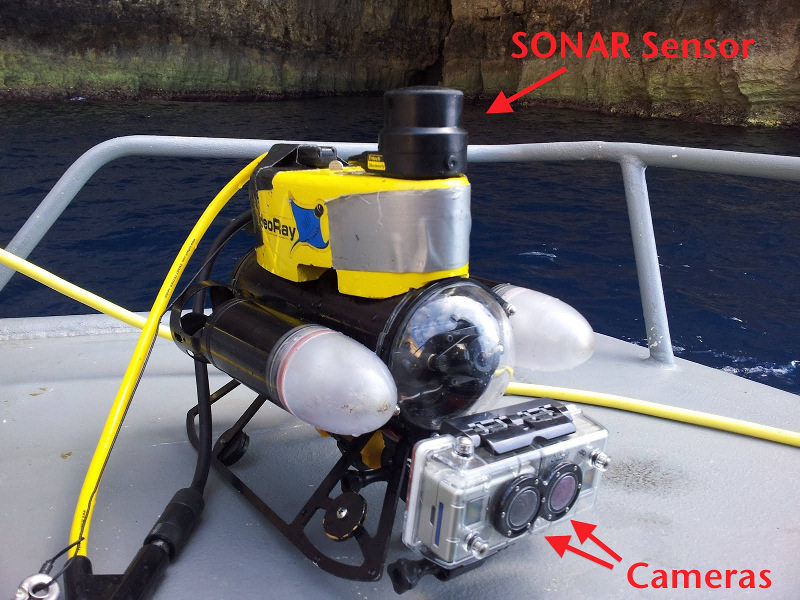
\epsfig{file = pics/ROV.jpg, width = 7cm}}
   \caption{Hardware setup, consisting of a Tritech SeaSprite sonar sensor and two vertically aligned HD GoPro cameras mounted on a VideoRay Pro III Micro ROV.}
  \label{fig:ROV}
 \end{figure}

While the ROV is navigating a cistern, two high-definition (HD) cameras mounted to the bow in a waterproof casing are triggered to synchronously capture images every two(?) seconds. The cameras are vertically aligned so as to minimize image disparity in the vertical direction. Due to occlusions from sediment and drifting objects uplifted by the ROV's thrusters, the camera images are often obscured, making conventional scan matching algorithms insufficient for disparity map generation (maybe this detail goes in Tim's section? possibly even in intro and/or abstract).

\section{\uppercase{Gross sonar Model Reconstruction}}
\label{sec:reconstruction}

%Discuss sonar models/how they are generated in our situation. More focused on the robotics aspect, rather than the details of Jeff and Billy's projects.

\noindent In this section we provide a background detailing the approach to rough geometry model generation from sonar input. Zoe" might be best at this... I think we just want to summarize it very fast and without too much detail so that we have more room for the stereo stuff. I tried to summarize section~\ref{sec:data} briefly as well, but perhaps we can shorten it a bit if we need more room. Mention that we extrapolate the near-ground scan plane into 3D in most cases, rather than having true 3D maps.

\begin{figure*}[!ht]
   \vspace{-0.2cm}
   \centering{
      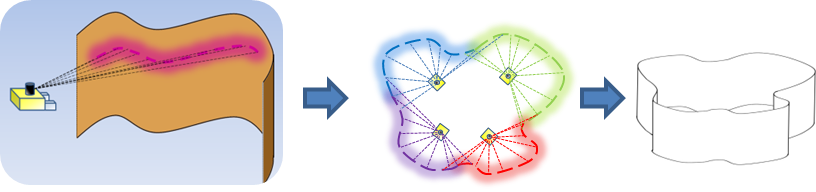
\epsfig{file = pics/1.png, width = 0.9\textwidth}}
   \caption{How we generate meshes from sonar models.}
  \label{fig:meshgen}
 \end{figure*}

\section{\uppercase{Fine Detail Additions Via Stereoscopic Depth Extraction}}
\label{sec:detail}

\noindent In this section we describe our approach towards the addition of fine details to the gross sonar models produced in Section~\ref{sec:reconstruction}. 

%Discuss why this is necessary. Discuss a system level overview of the process (more in depth than in introduction).

\subsection{Disparity Map Generation}

%Tim will write this one.

\noindent

\begin{figure*}[!ht]
   \vspace{-0.2cm}
   \centering{
      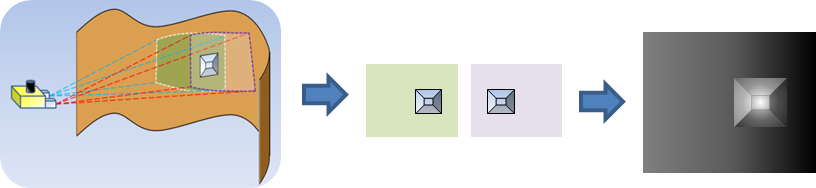
\epsfig{file = pics/2.png, width = 0.9\textwidth}}
   \caption{How we generate disparity maps from images.}
  \label{fig:dispgen}
 \end{figure*}

\subsubsection{Calibration}
\label{subsec:calibration}

%Never really got resolved. In my shaders I am still using an arbitrary scale factor. The calibration is possible... but I don't think it would get us anything that looks better than changing that scale factor by eye. This is because we were so inaccurate with our lasers/calibration on site. Perhaps we can discuss how to calibrate, but mention that we did not do it because guessing looks better.

\begin{figure}[!h]
	\centering
		\subfigure[Left camera image]{\label{left}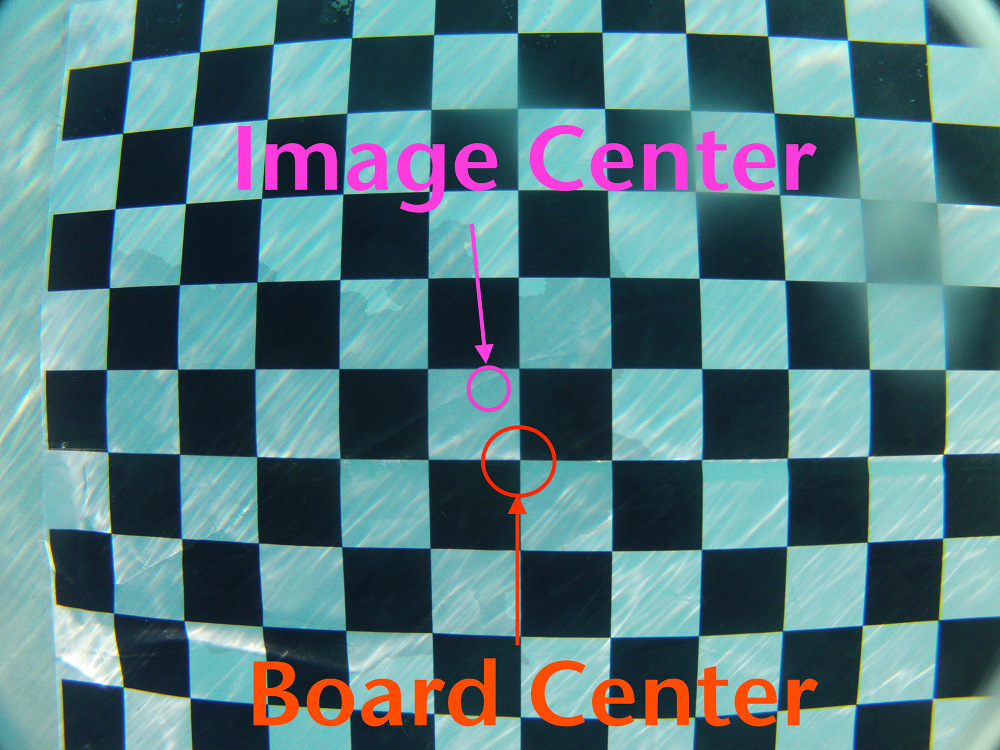
\epsfig{file = pics/calibrateL.jpg, width = 3.5cm}}
		\quad %space between images
		\subfigure[Right camera image]{\label{right}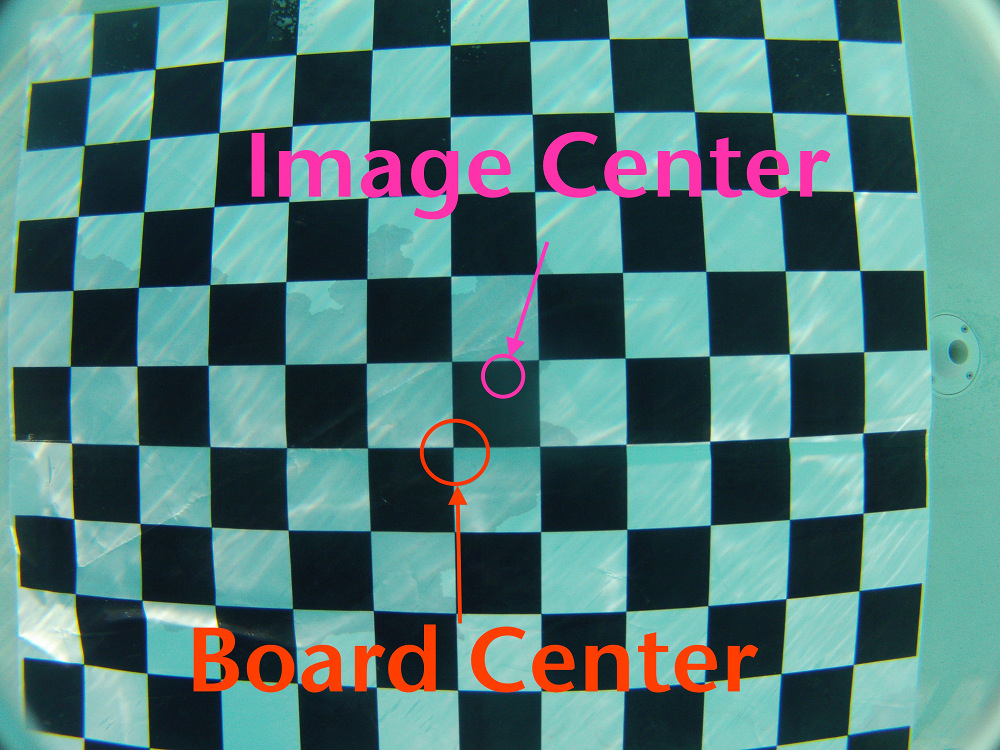
\epsfig{file = pics/calibrateR.jpg, width = 3.5cm}}
		\caption{calibration pics. Probably won't include but just in case.}
		\label{calibrate}
\end{figure}

\noindent 

\subsection{Projective Texturing}

%Describe how projective texturing works, describe how vertices are selected, describe phantom texture vs. displayed texture, then jump into math mode.

%Explains the method implemented to displace vertices. Discuss the use of a phantom texture to displace vertices, and the use of a photograph texture overlaid on the same wall segment. Discuss why displacing along toProjector is better than displacing along normal (graphic would be helpful). 

%Computation of plane eqs, acquire list of vertices contained within frustum, shader texturing. Explain why $\begin{Vmatrix}C\end{Vmatrix}$ is correct, talk about blending, explain how to determine whether vertex lies within frustum and how to texture map.

\noindent In order to add fine details to the gross sonar generated mesh, we establish projective texturing. Rather than implementing (traditional? is there a better word?) texturing, projective texturing is utilized because of its ability to properly simulate an ROV as a point particle with the ROV's view frustum modeled as six implicit plane equations. This similarity enables a 'copy paste' method of texturing, where the ROV captures an image of an organic feature in a cistern, and a projector casts the image from the same relative position onto the a gross sonar reconstruction (Figures~\ref{fig:dispgen},~\ref{fig:projtex}). 

OpenGL and OpenGL Shading Language (GLSL) graphics libraries are utilized to establish projective texturing, the latter being used to create shaders - small programs run per-vertex directly on the GPU. The shaders are programmed to selectively alter rendered vertex information, such as position (vertex shader) and color (fragment shader). The combination of projective texturing and stereoscopic imaging enables us to project a disparity map onto a surface, and selectively displace vertices along the vector from the vertex to the projector according to the color value of the textured disparity map. 

A projector is simulated by establishing position and plane equations for a view frustum based on the position and orientation of the ROV when the projected images were captured in a cistern.  We define $\mathbf{J} = \{\mathbf{j}_{1},\dots,\mathbf{j}_{N}\}$ to be the set of projectors casting textures onto the gross surface reconstruction. Each projector, $\mathbf{j}_{n} = ((\mathbf{j}_{n_{x}}^{pos},\mathbf{j}_{n_{y}}^{pos},\mathbf{j}_{n_{z}}^{pos}), \langle \mathbf{j}_{n_{x}}^{look},\mathbf{j}_{n_{y}}^{look},\mathbf{j}_{n_{z}}^{look}\rangle ^{\mathrm{T}})$, is uniquely defined by its position in 3D space, and a look vector orthonormal to the projector's viewport (Figure~\ref{fig:frustum}). All projectors have a pre-calibrated Field Of View (FOV) mimicking the compound FOV produced by the GoPro camera and waterproof housing lenses. The ROV is not equipped with roll thrusters, allowing us to ignore the possibility of a tilted camera frustum (i.e. the projector's right facing vector will always lie in the horizontal plane). Implicit plane equations modeling the projector view frustums in the form $Ax + By + Cz + D = 0$ are resolved using the clip space approach in [CITATION NEEDED], where $\langle A, B, C\rangle ^ {\mathrm{T}}$ is the plane's normal vector and  $(x, y, z)$ is a point on the plane.

\begin{align}
\nonumber %Left plane
&\lbrack A \hspace{3pt} B \hspace{3pt} C \hspace{3pt} D \rbrack^\mathrm{T}_{Left} \hspace{-15pt} &= \hspace{10pt}&\lbrack \chi_{11} \cdots \chi_{41} \rbrack^\mathrm{T} + \lbrack \chi_{14} \cdots \chi_{44} \rbrack^\mathrm{T}
\\
\nonumber %Right plane
&\lbrack A \hspace{3pt} B \hspace{3pt} C \hspace{3pt} D \rbrack^\mathrm{T}_{Right} \hspace{-15pt} &= -&\lbrack \chi_{11} \cdots \chi_{41} \rbrack^\mathrm{T} + \lbrack \chi_{14} \cdots \chi_{44} \rbrack^\mathrm{T}
\\
\nonumber %Top plane
&\lbrack A \hspace{3pt} B \hspace{3pt} C \hspace{3pt} D \rbrack^\mathrm{T}_{Top} \hspace{-15pt} &= \hspace{10pt}&\lbrack \chi_{12} \cdots \chi_{42} \rbrack^\mathrm{T} + \lbrack \chi_{14} \cdots \chi_{44} \rbrack^\mathrm{T}
\\
\nonumber %Bottom plane
&\lbrack A \hspace{3pt} B \hspace{3pt} C \hspace{3pt} D \rbrack^\mathrm{T}_{Bot} \hspace{-15pt} &= -&\lbrack \chi_{12} \cdots \chi_{42} \rbrack^\mathrm{T} + \lbrack \chi_{14} \cdots \chi_{44} \rbrack^\mathrm{T}
\\
\nonumber %Near plane
&\lbrack A \hspace{3pt} B \hspace{3pt} C \hspace{3pt} D \rbrack^\mathrm{T}_{Near} \hspace{-15pt} &= \hspace{10pt}&\lbrack \chi_{13} \cdots \chi_{43} \rbrack^\mathrm{T} + \lbrack \chi_{14} \cdots \chi_{44} \rbrack^\mathrm{T}
\\
\nonumber %Far plane
&\lbrack A \hspace{3pt} B \hspace{3pt} C \hspace{3pt} D \rbrack^\mathrm{T}_{Far} \hspace{-15pt} &= -&\lbrack \chi_{13} \cdots \chi_{43} \rbrack^\mathrm{T} + \lbrack \chi_{14} \cdots \chi_{44} \rbrack^\mathrm{T}
\\
\end{align}

\begin{figure}[!h]
   \vspace{-0.2cm}
   \centering{
      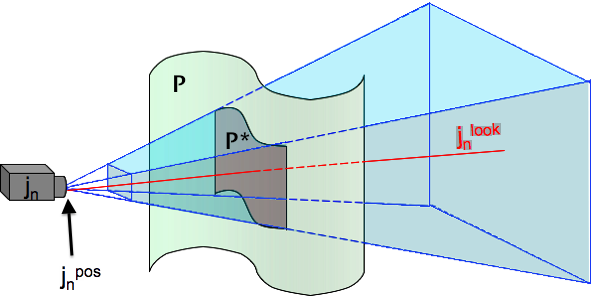
\epsfig{file = pics/frustum.png, width = 7cm}}
   \caption{Frustum and viewport.}
  \label{fig:frustum}
 \end{figure}

Next, for each projector, all faces in the mesh are passed through a view frustum culling filter in order to produce a list of faces contained within the frustum. We define $\mathbf{P} = \{\mathbf{p}_{1},\dots,\mathbf{p}_{M}\}$ to be the set of vertices contributing to the gross sonar reconstructed mesh. Each vertex, $\mathbf{p}_{n} =  (\mathbf{p}_{m_{x}},\mathbf{p}_{m_{y}},\mathbf{p}_{m_{z}})$, is defined by its position in 3D space. Additionally, we define $\mathbf{F} = \{\mathbf{f}_{1},\dots,\mathbf{f}_{Q}\}$ as the set of faces in the mesh. Each face, $\mathbf{f}_{q} = (\mathbf{p}_{\alpha}, \mathbf{p}_{\beta}, \mathbf{p}_{\gamma})$, is comprised of three vertices. We begin with a (un-memory-intensive... find another way to phrase - perhaps list big O notation?) preliminary cull which discards faces if their bounding sphere is outside of the projector's view frustum. Since frustum planes are modeled implicitly with normal vectors pointing into the frustum, if the signed distance from the face's center to the frustum plane, $\delta_{center}$, is less than the negative of the face's bounding sphere's radius, then the face's bounding sphere is entirely outside of the view frustum. In this case the face is immediately culled. $\delta_{center}$ is computed as follows,
%
\begin{equation}
\delta_{center} = \frac{Ax + By + Cz + D}{3 \begin{Vmatrix} \langle A, B, C \rangle \end{Vmatrix}},
\end{equation}

where
\begin{equation}
(x, y, z) = \left(\sum\limits_{\forall \mathbf{p}_{m} \in \mathbf{f}_{q}} \mathbf{p}_{m_{x}}, \sum\limits_{\forall \mathbf{p}_{m} \in \mathbf{f}_{q}} \mathbf{p}_{m_{y}}, \sum\limits_{\forall \mathbf{p}_{m} \in \mathbf{f}_{q}} \mathbf{p}_{m_{z}}\right)
\end{equation}

Once faces are passed through the preliminary culling filter, a more memory-intensive (if you do list big O for prev cull, list it for this one too) thorough cull is executed in order to remove the small number of faces that lie entirely outside of the frustum, but whose bounding spheres are still intersected by the frustum plane.  To accomplish this, the signed distances from each vertex in the face to the frustum plane, $\delta_{\alpha}$, $\delta_{\beta}$, and $\delta_{\gamma}$, are individually computed. If $\delta_{\alpha}$, $\delta_{\beta}$, and $\delta_{\gamma}$ are all less than zero, the face is culled. $\delta_{\alpha}$, $\delta_{\beta}$, and $\delta_{\gamma}$ are computed as follows,
%
\begin{equation} % fix this... shitty eqn
\delta_{\alpha, \beta, \gamma} = \frac{Ax + By + Cz + D}{\begin{Vmatrix} \langle A, B, C \rangle \end{Vmatrix}},
\end{equation}

where
\begin{align}
\nonumber
(x, y, z)_{\alpha} &= (\mathbf{p}_{\alpha_{x}}, \mathbf{p}_{\alpha_{y}}, \mathbf{p}_{\alpha_{z}})\\
\nonumber
(x, y, z)_{\beta} &= (\mathbf{p}_{\beta_{x}}, \mathbf{p}_{\beta_{y}}, \mathbf{p}_{\beta_{z}})\\
(x, y, z)_{\gamma} &= (\mathbf{p}_{\gamma_{x}}, \mathbf{p}_{\gamma_{y}}, \mathbf{p}_{\gamma_{z}})
\end{align}


With faces lying outside of the projector view frustums culled, the vertices in the remaining faces are added to a trimmed set, $\mathbf{P}^{*}\subset \mathbf{P}$, whose members are sent to the vertex and fragment shaders (i.e. to the GPU) to be and displaced and textured in accordance with the generated disparity map and left camera image, respectively (Figure~\ref{fig:frustum}). $\mathbf{P}$ is also sent to the GPU so that the portions of the mesh that are not displaced or textured are still rendered.

\subsection{Vertex Displacement}

NOT FINISHED FROM HERE ON
 Let $C = \langle C_{r},C_{g},C_{b}\rangle ^\mathrm{T}$ be a three component vector containing the RGB color value of the projected texture at $\mathbf{p}_{m}$, and $\vec{b} = \mathbf{j}_{n} - \mathbf{p}_{m}$ be the vector originating at the vertex $\mathbf{p}_{m}$ and pointing towards the projector $\mathbf{j}_{n}$. Then,
\begin{equation}
\mathbf{p}_{m}' = \left \{ 
\begin{array}{ll}
\mathbf{p}_{m} + (\vec{b} \begin{Vmatrix}C\end{Vmatrix} S) & \text{if} \quad \mathbf{p}_{m} \in \mathbf{P}^{*}\\
\mathbf{p}_{m} & \text{if} \quad \mathbf{p}_{m} \notin \mathbf{P}^{*}
\end{array}\right.
\label{eq:displace}
\end{equation}

where $\mathbf{p}_{m}'$ is the displaced vertex position and $S$ is the scale factor determined in Section~\ref{subsec:calibration}. 
\begin{figure*}[!ht]
   \vspace{-0.2cm}
   \centering{
      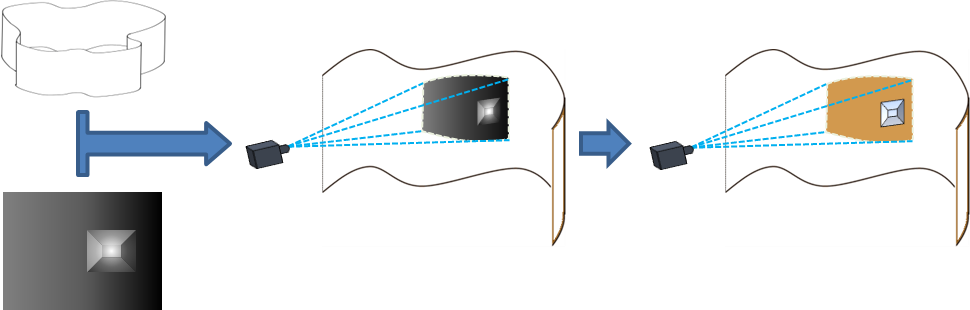
\epsfig{file = pics/3.png, width = 0.9\textwidth}}
   \caption{How we project textures and displace vertices yo.}
  \label{fig:projtex}
 \end{figure*}

\section{\uppercase{Results}}
\label{sec:results}

\noindent Description and noticeable features in the output, with pictures/screen caps. 

\begin{figure}[!h]
	\centering
		\subfigure[Left camera image]{\label{left}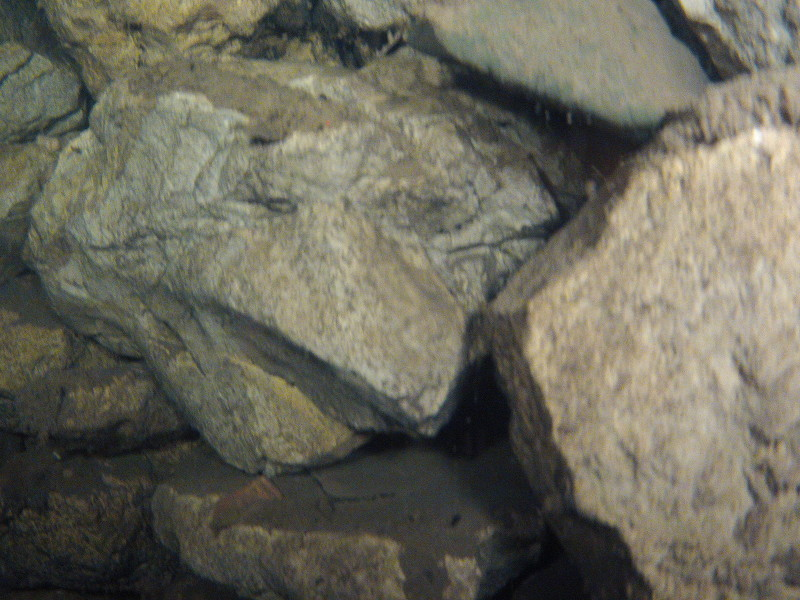
\epsfig{file = pics/left.jpg, width = 3cm}}
		\quad %space between images
		\subfigure[Right camera image]{\label{right}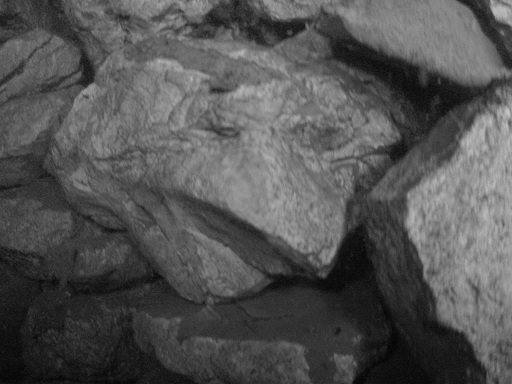
\epsfig{file = pics/right.jpg, width = 3cm}}\\%new line
		\medskip
		\subfigure[Disparity map as seen by left camera]{\label{disparitymap}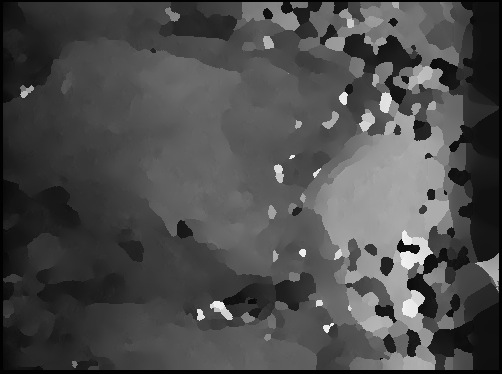
\epsfig{file = pics/disparity.jpg, width = 3cm}}
		\caption{We will replace this pics when Tim gets us some boss map di\$parity map\$\$\$}
		\label{disparity}
\end{figure}

\section{\uppercase{Conclusion and Future Work}}
\label{sec:conclusion}

\noindent Summary and future work.

\bibliographystyle{apalike}
{\small
\bibliography{Stereo}}

\end{document}

